%\setcounter{chapter}{0} % permette di impostare un numero di capitolo differente da quello di default
\chapter{Evoluzione dei Game Engine}
\label{cap:evoluzione}

\section{Background storico}
Nell'ultimo decennio l'industria videoludica si è evoluta notevolmente, soprattutto nel modo in cui i videogiochi vengono realizzati. Oggi infatti, per realizzare un gioco non dobbiamo più scrivere migliaia di righe di codice ma possiamo pensare e lavorare tramite interfacce grafiche e componenti di alto livello. Questo modello di sviluppo è strettamente correlato all'evoluzione dei Game Engine.

L'origine del concetto di Game Engine è da ricercare a metà degli anni '90, principalmente in ambito di giochi 3D o FPS, quando la casa produttrice \emph{id Software} rilasciò un comunicato stampa per annunciare l'uscita di DOOM~\cite{article:hall1992doom}.
Il documento prometteva che il gioco avrebbe «spinto i limiti di ciò che si pensava fosse possibile realizzare su un computer 386sx o migliore», riassumendo diverse innovazioni e tecnologie adottate per implementarlo e, soprattutto, parlava di \emph{DOOM engine}. Inoltre, l'articolo presentava DOOM come un \emph{Open Game}, affermando che la casa produttrice avrebbero fornito la tecnologia ed il supporto per utilizzarla a chiunque l'avesse richiesto.

Questo fu un momento storico molto importante che diede una svolta all'industria videoludica, in quanto per la prima volta si parlò di Game Engine e della separazione dei vari componenti e ambiti nella realizzazione dei giochi. Negli anni successivi il termine è diventato sempre più utilizzato per indicare l'ambiente di sviluppo per progettare e costruire videogiochi (e non solo), composto da vari componenti: rendering grafico, motore fisico, suoni, animazioni, scripting, ecc.
Infatti, analizzando il grafico Google in Figura~\ref{fig:game-engine-google-search} notiamo subito come le ricerche per ``game engine'' si siano impennate proprio negli anni immediatamente seguenti alla pubblicazione di DOOM~\cite{article:lowood2014game}. 
Da quel momento diverse case produttrici hanno deciso di creare un'implementazione proprietaria al fine di utilizzare il game engine per lo sviluppo dei propri videogiochi, mentre società quali ad esempio \emph{Epic Games} e \emph{Unity Technologies} si sono concentrate sulla creazione di un'architettura il più completa possibile e con interfacce user-friendly, che potesse essere utilizzata da tutti, fornendo la relativa documentazione.

\begin{figure}[!ht]
    \centering
    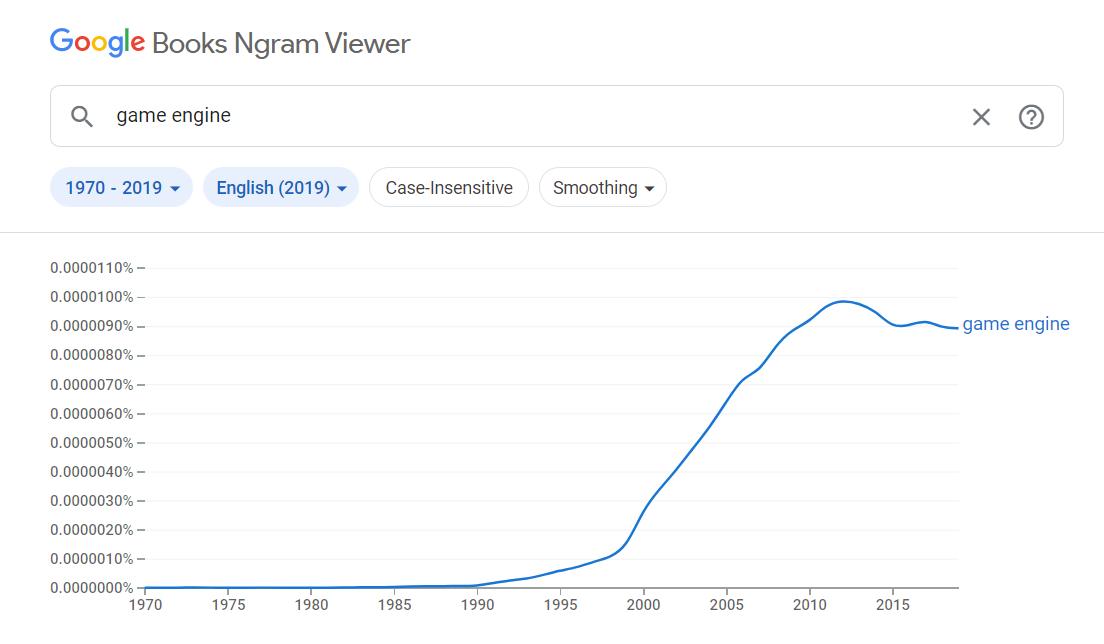
\includegraphics[width=0.95\columnwidth]{gfx/imgs/chapter1/GameEngineGoogleSearch.png}
    \caption{Google Ngram Viewer: ricerche per ``game engine'' negli anni 1970-2019.}
    \label{fig:game-engine-google-search}
\end{figure}

% Game Engine role in game development
%https://momentsonline69.medium.com/the-role-of-game-engines-in-video-game-development-2f1e42e298aa#_=_

\section{Modelli architetturali}
I modelli architetturali adottati nello sviluppo di videogiochi e dai game engine sono riassumibili in tre principali categorie: \emph{inheritance model}, \emph{component-based model} ed \emph{entity component system} (tipicamente abbreviato con ECS).

\subsection{Inheritance model}
Questo pattern è il più tradizionale (molto usato negli anni '90), ed è tipico della programmazione orientata agli oggetti, in cui solitamente è presente una classe, chiamata appunto GameObject, che rappresenta il nodo radice e tutte le classi sottostanti ereditano dati e logica da quest'ultima, creando catene gerarchiche di lunghezza variabile.

L'inheritance model è molto intuitivo e ci permette di semplificare la definizione e la realizzazione di tipi di dato simili, fornendo inoltre la possibilità di sovrascrivere i metodi delle superclassi. Il problema principale di questo modello consiste nel fatto che man mano che i livelli della gerarchia crescono, solitamente perché dobbiamo aggiungere delle entità o delle funzionalità nel gioco, la complessità del codice aumenta con la conseguente diminuzione di riusabilità, flessibilità e, soprattutto, performance. Pertanto, è perfetto per applicazioni e giochi di piccole dimensioni e con poche classi o regole semplici, ma non è assolutamente un modello scalabile~\cite{phd:romeoanalysis}.

\begin{figure}[!ht]
    \centering
    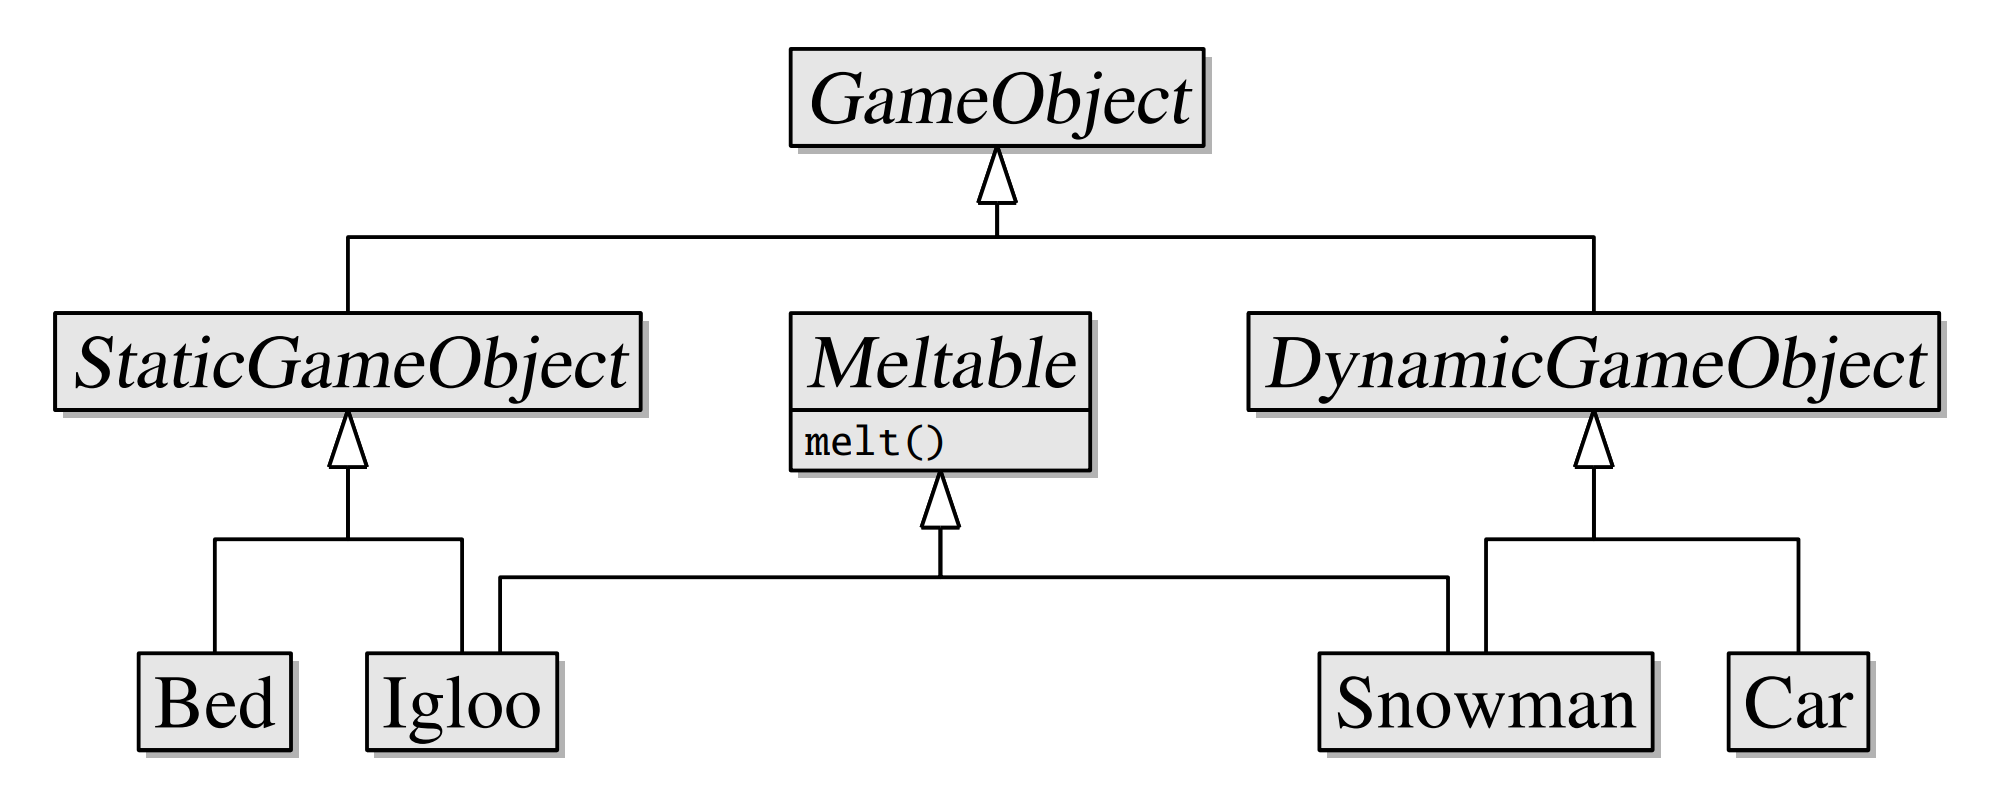
\includegraphics[width=0.95\columnwidth]{gfx/imgs/chapter1/InheritanceModel.png}
    \caption{Esempio: inheritance model~\cite{article:game-architecture-models}.}
    \label{fig:inheritance-model}
\end{figure}

\begin{figure}[!ht] 
    \centering
    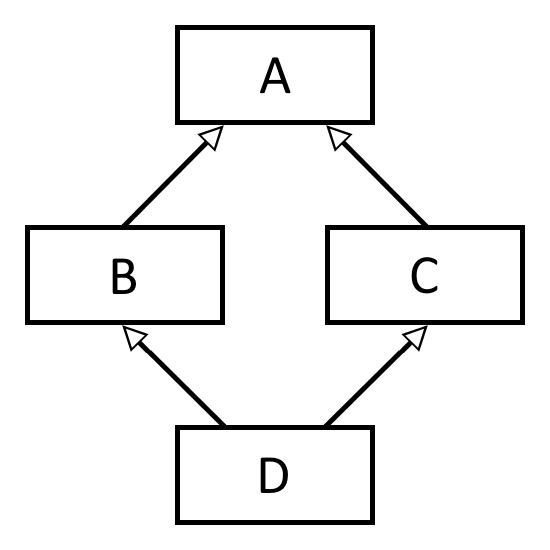
\includegraphics[width=0.50\columnwidth]{gfx/imgs/chapter1/DiamondProblem.png}
    \caption{Problema del diamante.}
    \label{fig:diamond-problem}
\end{figure}

\paragraph{Problema del diamante}
Fra i diversi problemi dell'Inheritance Model, il più famoso è sicuramente il \emph{problema del diamante}, dovuto all'ereditarietà multipla. Se due classi B e C ereditano da una stessa superclasse A, ed una classe D eredita da entrambe B e C, abbiamo ambiguità nel caso la classe D chiamasse un metodo definito in A, in quanto avrebbe due implementazioni diverse (vedi Figura~\ref{fig:diamond-problem}). Per aggirare questo problema, prendendo come esempi i linguaggi \Csh{} e Java, è stato imposto un vincolo secondo cui una classe può ereditare le interfacce da più classi base, ma i metodi ed i dati solamente da una di esse~\cite{article:diamond-problem,itwiki:99605337}.

\subsection{Component-based model}
In un modello basato sui componenti, la gerarchia dei GameObject viene appiattita ad un singolo livello base di GameObject. Quest'ultimo contiene una lista di classi che ne realizzano il comportamento, chiamate componenti.
In questo modo, i GameObject vengono disaccoppiati dal comportamento ed il modello diventa più mantenibile e flessibile, permettendo di creare nuovi tipi di GameObject sfruttando l'aggiunta di ulteriori componenti. Infatti, con questo modello il tipo di un GameObject non è più definito dalla gerarchia di classi a cui appartiene, ma dalla lista di componenti che possiede.

\begin{figure}[!ht]
    \centering
    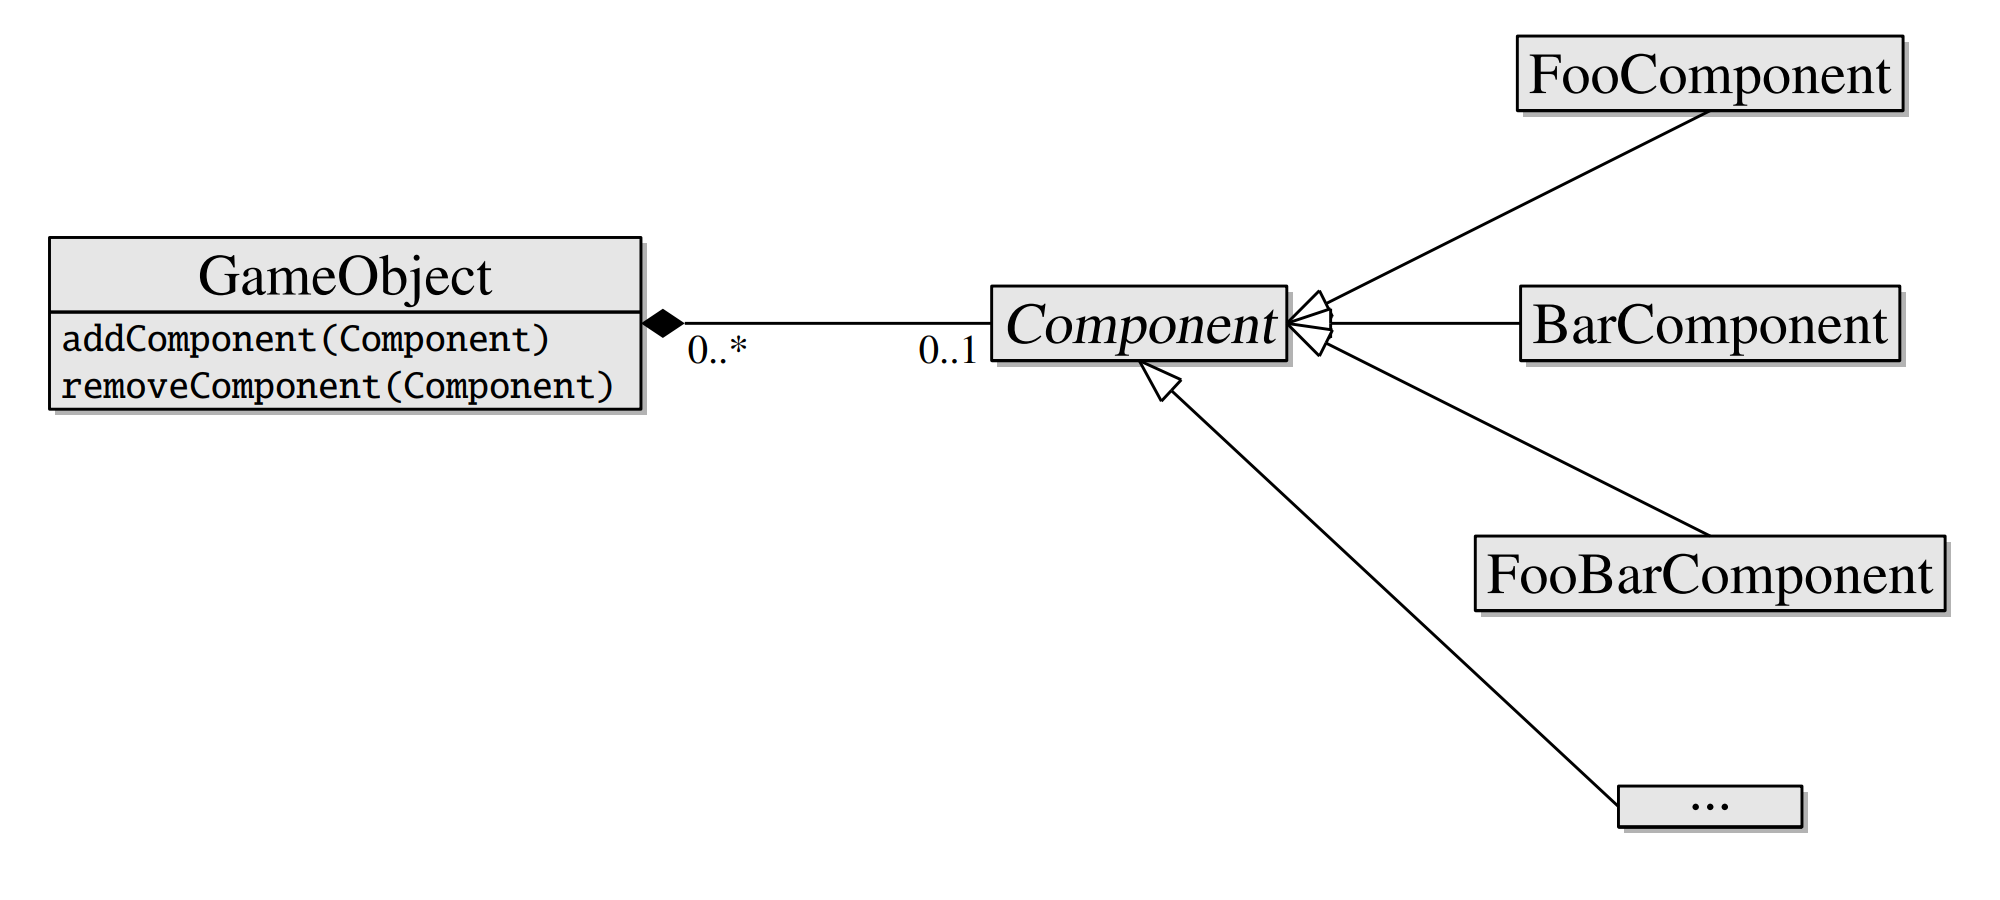
\includegraphics[width=0.95\columnwidth]{gfx/imgs/chapter1/ComponentBasedModel.png}
    \caption{Esempio: component-based model~\cite{article:game-architecture-models}.}
    \label{fig:component-based-model}
\end{figure}

Rispetto al precedente approccio, il component-based model possiede diversi vantaggi, fra cui:
\begin{itemize}
    \item Scalabilità in termini di numero di tipi di GameObject e di comportamento realizzabile per ognuno di essi. 
    \item Modularità dei componenti.
    \item Flessibilità e manutenibilità.
\end{itemize}

Tuttavia, le API dei componenti non sono flessibili ed un loro cambiamento richiede la modifica di tutti i componenti. Infine, i maggiori problemi di questo approccio sono legati all'utilizzo inefficiente di CPU, cache, ed accesso alla memoria~\cite{article:game-architecture-models}.

\paragraph{Utilizzo risorse, CPU e cache}
Sebbene sia un modello migliore del precedente, rimangono comunque molti aspetti che influiscono negativamente sulle prestazioni. In particolare, riguardo l'utilizzo delle risorse, sia inheritance model che component-based model non sono particolarmente ``hardware-friendly''.

Negli ultimi anni, i processori prodotti sono arrivati ad una sorta di velocità limite del clock oltre la quale, per vari motivi~\cite{article:cpu-speed-cap}, non ha più senso spingersi~\cite{article:cpu-evolution}. Di conseguenza, la soluzione migliore per continuare ad ottenere maggiore potenza nelle CPU, è stata quella di aggiungere core (vedi Figura~\ref{fig:cpu-evolution}). Tuttavia, nello sviluppo dei videogiochi spesso solamente uno, massimo due core, vengono sfruttati molto intensamente. Questo solitamente accade perché motori di gioco basati su questo modello architetturale mal supportano la programmazione multithreading. Di conseguenza, il carico sulla CPU non viene bilanciato adeguatamente.

\begin{figure}[!ht]
    \centering
    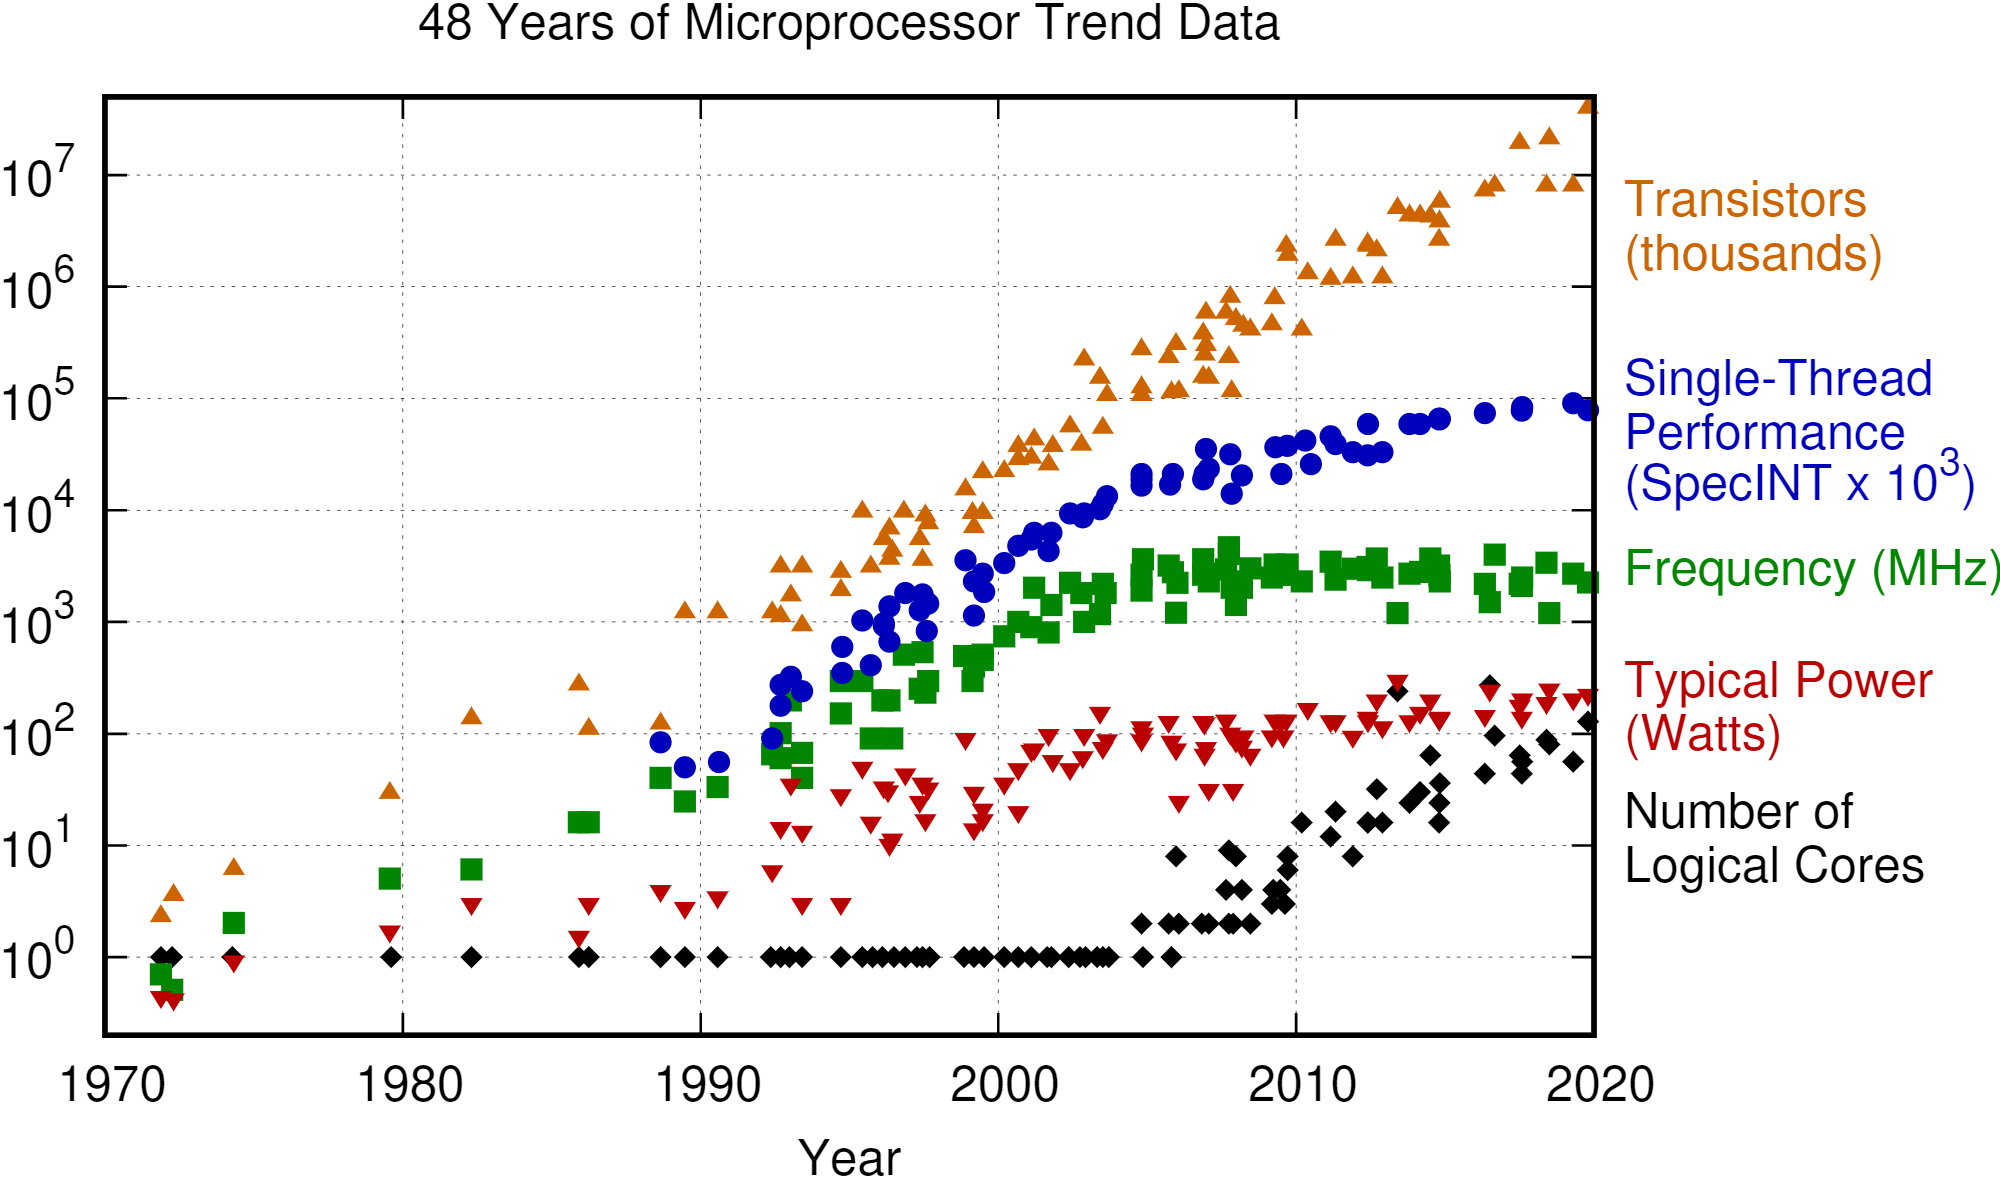
\includegraphics[width=0.95\columnwidth]{gfx/imgs/chapter1/CPUEvolution.png}
    \caption{Evoluzione delle CPU negli ultimi decenni~\cite{repo:cpu-evolution-data}. Nel grafico possiamo notare come la velocità dei transistor (verde) sia rimasta praticamente la stessa negli ultimi 20 anni, mentre il numero di core (nero) abbia continuato ad aumentare in modo pressoché uniforme.}
    \label{fig:cpu-evolution}
\end{figure}

Dunque, il limite principale per la maggior parte dei giochi e delle applicazioni è, e probabilmente sarà almeno per qualche anno, l'utilizzo ottimizzato delle risorse e l'accesso alla memoria. In particolare, ci serve l'impegno del programmatore per strutturare il codice in modo efficiente (ad esempio sfruttando design pattern e design principle) al fine di evitare cache misses e bottleneck. Per approfondire questi argomenti si può fare riferimento a~\cite{article:drepper2007every}.

\subsection{Unity}
Il game engine di \emph{Unity Technologies} è costruito sul component-based model e il suo core è scritto nei linguaggi di programmazione C e C\texttt{++}. Per quanto riguarda lo sviluppo di giochi basati su questo motore, agli sviluppatori finali vengono fornite diverse librerie scritte in linguaggio \Csh. Tali librerie funzionano da wrapper esterno del core del motore di gioco Unity, e sono utilizzate per la scrittura della logica di gioco. In particolare, l'architettura di Unity si basa su due classi fondamentali: 

\begin{enumerate}
    \item \emph{GameObject}. Rappresenta le entità, ovvero gli oggetti presenti nella scena (il mondo/livello in cui esistono)~\cite{doc:unity-gameobjects}.
    \item \emph{MonoBehaviour}. I componenti che realizzano il comportamento delle entità. Solitamente l'implementazione del comportamento avviene tramite il metodo \verb|Update()|, il quale a runtime viene chiamato ad ogni frame~\cite{doc:unity-monobehaviour}.
\end{enumerate}

Il problema principale è l'utilizzo delle risorse, di conseguenza un'architettura di questo genere è perfetta per lo sviluppo di giochi Indie\footnote{Indie è l'abbreviazione del termine inglese \emph{independent} che, in questo caso, fa riferimento ai giochi sviluppati da un singolo programmatore o poche persone, non facenti parte di una software house.}, ma assolutamente inadatta allo sviluppo di applicazioni complesse.

\paragraph{Limiti dell'architettura classica di Unity}
Con \emph{architettura classica} intendiamo il modo tradizionale di sviluppo delle applicazioni su Unity, ovvero tramite la creazione di GameObject o Prefab e l'inserimento di questi in una scena, allegandoci dei MonoBehaviour per fargli fare qualcosa. I MonoBehaviour sono script che ereditano dalla classe \verb|MonoBehaviour|. Il limite di questa soluzione è che introduce un forte legame tra i dati ed il loro processamento (tutto si trova nella stessa classe all'interno del medesimo script). Inoltre, in questo modo abbiamo una stretta dipendenza dai tipi riferimento, i quali gravano molto sulle performance, in quanto indirizzano dei dati che sono sparpagliati in memoria.

Un GameObject è un container che contiene diversi riferimenti ad altre aree di memoria, le quali potrebbero avere altri riferimenti e così via. Quando la CPU deve lavorare su un GameObject, se questo non è presente in cache dev'essere spostato in quest'ultima. Ma poiché è un tipo riferimento, l'operazione può diventare complessa e richiedere molto tempo. Inoltre, spesso ci si trova a processare più dati di quanti effettivamente ne servano.
Ad esempio, i GameObject in Unity devono necessariamente avere un componente \verb|Transform| allegato, che ne specifica la posizione, la rotazione e le dimensioni~\cite{doc:unity-transforms}. Però, matematicamente parlando, se volessimo semplicemente traslare un oggetto, tutto ciò che ci serve è la posizione attuale, la direzione e la velocità di movimento. Nel componente \verb|Transform| (Figura~\ref{fig:transform-class}) ci sono tantissimi altri dati superflui. Tuttavia, quando dobbiamo utilizzare un campo che si trova nel componente Transform, la CPU deve caricarlo tutto in memoria centrale, anche se ce ne serve solo una piccola parte. In questo modo sprechiamo tutto il potenziale delle cache più veloci che, avendo poca memoria, vengono riempite di dati inutili. Inoltre, con l'approccio classico non operiamo veramente su più di un thread. Tutto il processamento dei dati eseguito dai MonoBehaviour avviene in sequenza sul main thread (Figura~\ref{fig:traditional-data-processing}).

\SaveVerb{TransformTerm}|Transform|
\SaveVerb{UnityUnityEngineTerm}|Unity.UnityEngine|

\begin{figure}[!ht]
    \centering
    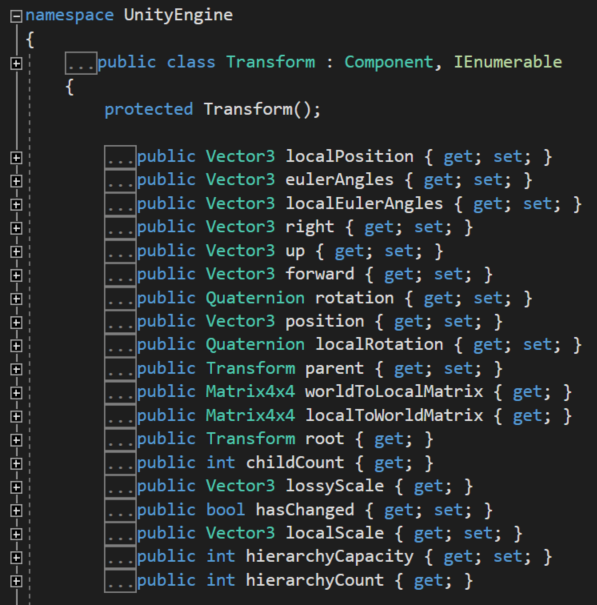
\includegraphics[width=0.64\columnwidth]{gfx/imgs/chapter1/TransformClassUnityEngine.png}
    \caption{Parte della classe \protect \UseVerb{TransformTerm} di \protect \UseVerb{UnityUnityEngineTerm}.}
    \label{fig:transform-class}
\end{figure}

\begin{figure}[!ht]
    \centering
    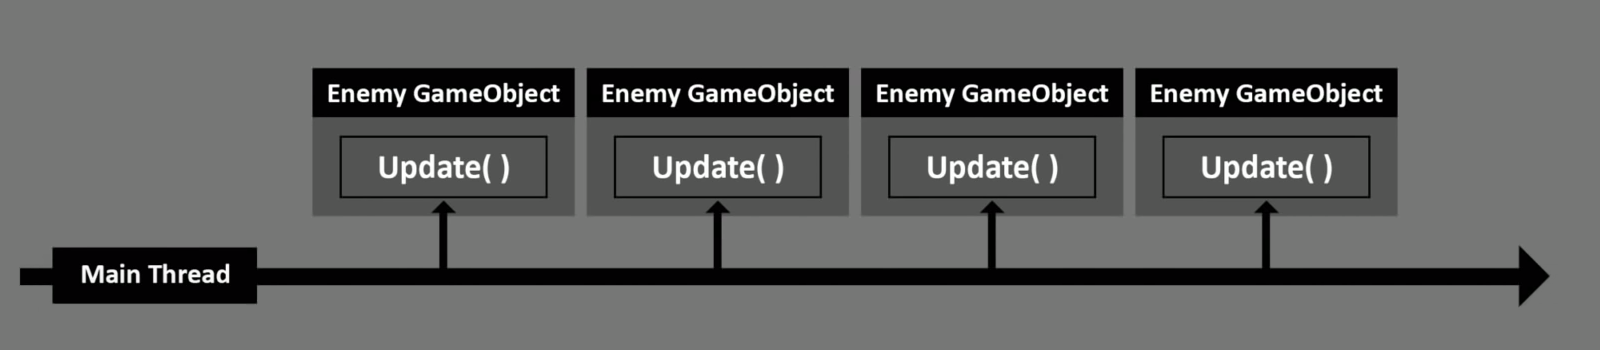
\includegraphics[width=0.90\columnwidth]{gfx/imgs/chapter1/MainThread.png}
    \caption{Processamento dei dati nel modello classico~\cite{youtube:differenze-unity-classico}.}
    \label{fig:traditional-data-processing}
\end{figure}

\subsection{Unreal Engine}
Come Unity, anche il game engine di \emph{Epic Games} è costruito sul component-based model ma, a differenza del primo, Unreal utilizza gli Actor al posto dei GameObject. Possiamo vedere gli Actor come interi oggetti o entità, che possiamo piazzare all'interno del livello di un mondo e possono avere dei componenti che realizzano il comportamento. Sia attori che componenti vengono aggiornati ogni frame tramite un'operazione chiamata \emph{ticking} (in contrapposizione al metodo \verb|Update()| in Unity), che permette di specificare se dev'essere attivata ad ogni frame oppure no~\cite{doc:unreal-architecture}.
Rispetto a Unity, Unreal ottimizza il component-based model, il quale risulta comunque limitato se comparato al modello basato su entità, di cui parleremo nella prossima sezione.

\subsection{Entity Component System}
Entity Component System (ECS) è un pattern architetturale di sviluppo del software che ha come obbiettivo la separazione dei dati dalla logica. Segue il principio del \emph{Composition over Inheritance}, secondo cui le classi dovrebbero realizzare il polimorfismo e il riutilizzo di codice tramite la composizione (contenendo riferimenti), piuttosto che ereditando da una classe padre. Questo ci permette appunto di ottenere maggiore separazione delle competenze e rende il codice flessibile, modulare e, di conseguenza, facilmente leggibile e riutilizzabile~\cite{article:composition-over-inheritance}. Inoltre, eliminando l'overhead generato dalle catene di ereditarietà e tramite l'utilizzo di un approccio data-oriented, ECS permette di raggiungere livelli molto elevati di prestazioni (fondamentali in un videogioco), massimizzando l'utilizzo delle risorse. Infatti, i componenti sono più leggeri e facili da memorizzare degli oggetti: per questo motivo possono essere memorizzati in aree di memoria continue (array) permettendoci di sfruttare al meglio le cache dei processori, in particolare quelle di primo e secondo livello, che sono le più veloci.

Come indica la sigla, ECS comprende tre principali concetti:
\begin{itemize}
    \item \textbf{Entities}. Le ``entità'' che popolano il gioco, che rappresentano un oggetto concreto nell'applicazione. Non contengono né dati né logica, ma sono composte da componenti piccoli, riusabili e generici.
    \item \textbf{Components}. I dati associati alle entità. I componenti immagazzinano i dati o lo stato, ma non contengono alcun tipo di logica. Ciò che caratterizza ECS e lo rende efficiente è il fatto che i componenti sono organizzati proprio per dati e non per entità.
    \item \textbf{Systems}. Realizzano il comportamento. I sistemi contengono la logica che modifica lo stato dei componenti. Ad esempio potremmo creare un sistema che ruota tutte le entità che hanno un componente ``RotateComponent''.
\end{itemize}


\section{Unity DOTS}
Per risolvere i problemi di performance legati al modello su cui si fondava il motore di gioco, nel 2018, Unity ha presentato una soluzione basata su un design orientato ai dati~\cite{book:data-oriented-design}: DOTS.

\emph{Data-Oriented Technology Stack} (DOTS) è un insieme di librerie realizzate dagli sviluppatori di Unity negli ultimi due anni, tutt'oggi in fase di sviluppo. Il loro scopo fu quello di rivoluzionare l'architettura del game engine facendo in modo che le prestazioni non venissero limitate dal modello su cui si basava. A tal proposito, nello stack sono stati inseriti diversi package, fra cui in particolare ECS e Job System, che permettono di risolvere i principali problemi della vecchia architettura, e NetCode, per rivoluzionare il modello networking.

Il Job System permette di sfruttare il multi-core processing tramite il multithreading, così da non caricare tutto il lavoro su uno o due core, ma distribuirlo uniformemente, sfruttando il più possibile anche gli altri core della CPU. Inoltre, il Job System gestisce da solo tutti i problemi legati al multithreading (scrivere codice thread-safe è difficile, dobbiamo evitare corse critiche, il context switching è costoso, ecc.), così che lo sviluppatore possa focalizzarsi sulla logica o altri aspetti del gioco.

ECS permette di organizzare meglio il codice separando i dati dalle funzionalità, garantendo diversi benefici:
\begin{itemize}
    \item Scrivere codice non performante con DOTS diventa difficile, proprio grazie al modello ECS su cui si basa, il quale è performante a propri (\emph{performance by default}).
    \item È facile scrivere codice altamente ottimizzabile e riutilizzabile.
    \item Permette di sfruttare al meglio l'architettura hardware su cui il codice esegue, in quanto i dati sono memorizzati per archetipo, in modo molto compatto ed efficiente. Come conseguenza, tutte le operazioni che esegue la CPU sui dati (fetching, caricamento, ecc.) sono velocizzate, massimizzando l'utilizzo delle risorse e riducendo i consumi~\cite{youtube:overview-ecs-job}.
\end{itemize}

\SaveVerb{RotationTerm}|Rotation|
\SaveVerb{TranslationTerm}|Translation|
\SaveVerb{LocalToWorldTerm}|LocalToWorld|

\begin{figure}[!ht]
    \centering
    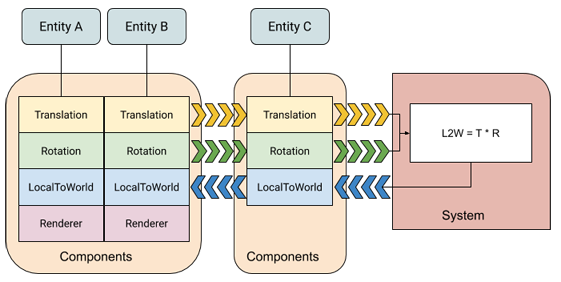
\includegraphics[width=0.90\columnwidth]{gfx/imgs/chapter1/ECSBlockDiagram.png}
    \caption{Esempio di funzionamento del pattern ECS: il sistema sulla destra prende in ingresso i componenti \UseVerb{TranslationTerm} e \UseVerb{RotationTerm} delle entità e aggiorna \UseVerb{LocalToWorldTerm} con il loro prodotto~\cite{doc:unity-entities-manual}.}
    \label{fig:ecs-example}
\end{figure}
Infine, NetCode fornisce un modello di networking a server autoritativo con server dedicato e predizione del client. Questo permette di ridurre al minimo la latenza, migliorando notevolmente l'esperienza di gioco. Di conseguenza, si presta molto bene ad essere utilizzato per la realizzazione di giochi che richiedono requisiti di lag minimi, quali ad esempio gli FPS.

Il resto della tesi è organizzato come segue.

\paragraph{Capitolo 2}
Introdurremo il package Entities, illustrando le API ed i costrutti fondamentali, spiegando com'è possibile realizzare il modello a Entity Component System in Unity. Inoltre, forniremo degli esempi, e spiegheremo le differenze sostanziali con l'architettura classica basata su GameObject e MonoBehaviour.

\paragraph{Capitolo 3}
Apriremo questo capitolo fornendo un background sulla realizzazione di videogiochi multiplayer, mostrando le principali topologie di rete, i protocolli utilizzati ed i problemi che si possono riscontrare. Dopodiché tratteremo il package Transport, che si occupa di sostituire le vecchie API di basso livello di UNet, ed infine il package NetCode, che assumerà particolare rilevanza soprattutto per il capitolo successivo.

\paragraph{Capitolo 4}
In questo capitolo mostreremo le funzionalità ed i passaggi utilizzati per realizzare il prototipo basato su DOTS. In particolare spiegheremo il significato e la funzione dei principali file implementati per il progetto.

\paragraph{Capitolo 5}
Effettueremo un'analisi qualitativa del prototipo realizzato e introdurremo un secondo prototipo, molto più semplice, che ci tornerà utile ai fini di testing e valutazione delle performance. Per farlo vedremo come utilizzare il Profiler Unity per ricavare informazioni riguardanti le prestazioni. 

\paragraph{Conclusioni e Sviluppi Futuri}
In questo capitolo trarremo le conclusioni, analizzando soprattutto i risultati ottenuti nel capitolo precedente e proponendo dei possibili sviluppi futuri.